\documentclass[class=book, crop=false]{standalone}
\usepackage[subpreambles=true]{standalone}
\usepackage{import}
\usepackage[ruled,vlined]{algorithm2e}

\usepackage{amsmath}
\usepackage{amssymb}
\usepackage[margin=1.2in]{geometry}
\usepackage[sorting = none,
            doi = true  %lesedato for url-adresse
            ]{biblatex} %none gir bibliografi i sitert rekkefølge
\addbibresource{reference.bib}
\usepackage{csquotes}
\usepackage{pgfplots}
\pgfplotsset{compat=1.15}

\begin{document}
\section{Problem description}
Solar power production occurs during day-time and is, not surprisingly controlled by the sun. Figure ?? shows a typical solar profile for a day. As photovoltaic modules become common in residential areas, they will grow to a size where they produce a significant amount of power that must be transported out on the grid. A consequence of this can can be that safety bounds for both voltage and line capacity are violated. A strategy for avoiding is called demand response. Albadi and El-Saadany give the following definition of demand response.\cite{demand_response_definition}

\begin{displayquote}
Demand response can be defined as the changes in electricity usage by end-use customers from their normal consumption patterns in response to changes in the price of electricity over time. Further, DR can be also defined as the incentive payments designed to induce lower electricity use at times of high wholesale market prices or when system reliability is jeopardized. DR includes all intentional electricity consumption pattern modifications by end-use customers that are intended to alter the timing, level of
instantaneous demand, or total electricity consumption.
\end{displayquote}


The idea is to modify the demand of electric power to follow the production profile of distributed energy resources (DER), such as solar power. The specific setup in this thesis is based on several assumptions for a hypothetical future power grid. The electrical power grid used is constructed by the International Council on Large Electric Systems (CIGRE) as a benchmark network that can be used for analysis of DER integration\cite{cigre}. The network is predefined in pandapower and can by defined with different renewable energy sources connected at different buses. The grid is visualised in figure \ref{fig:problem:cigre_network}. 

\begin{figure}[H]
    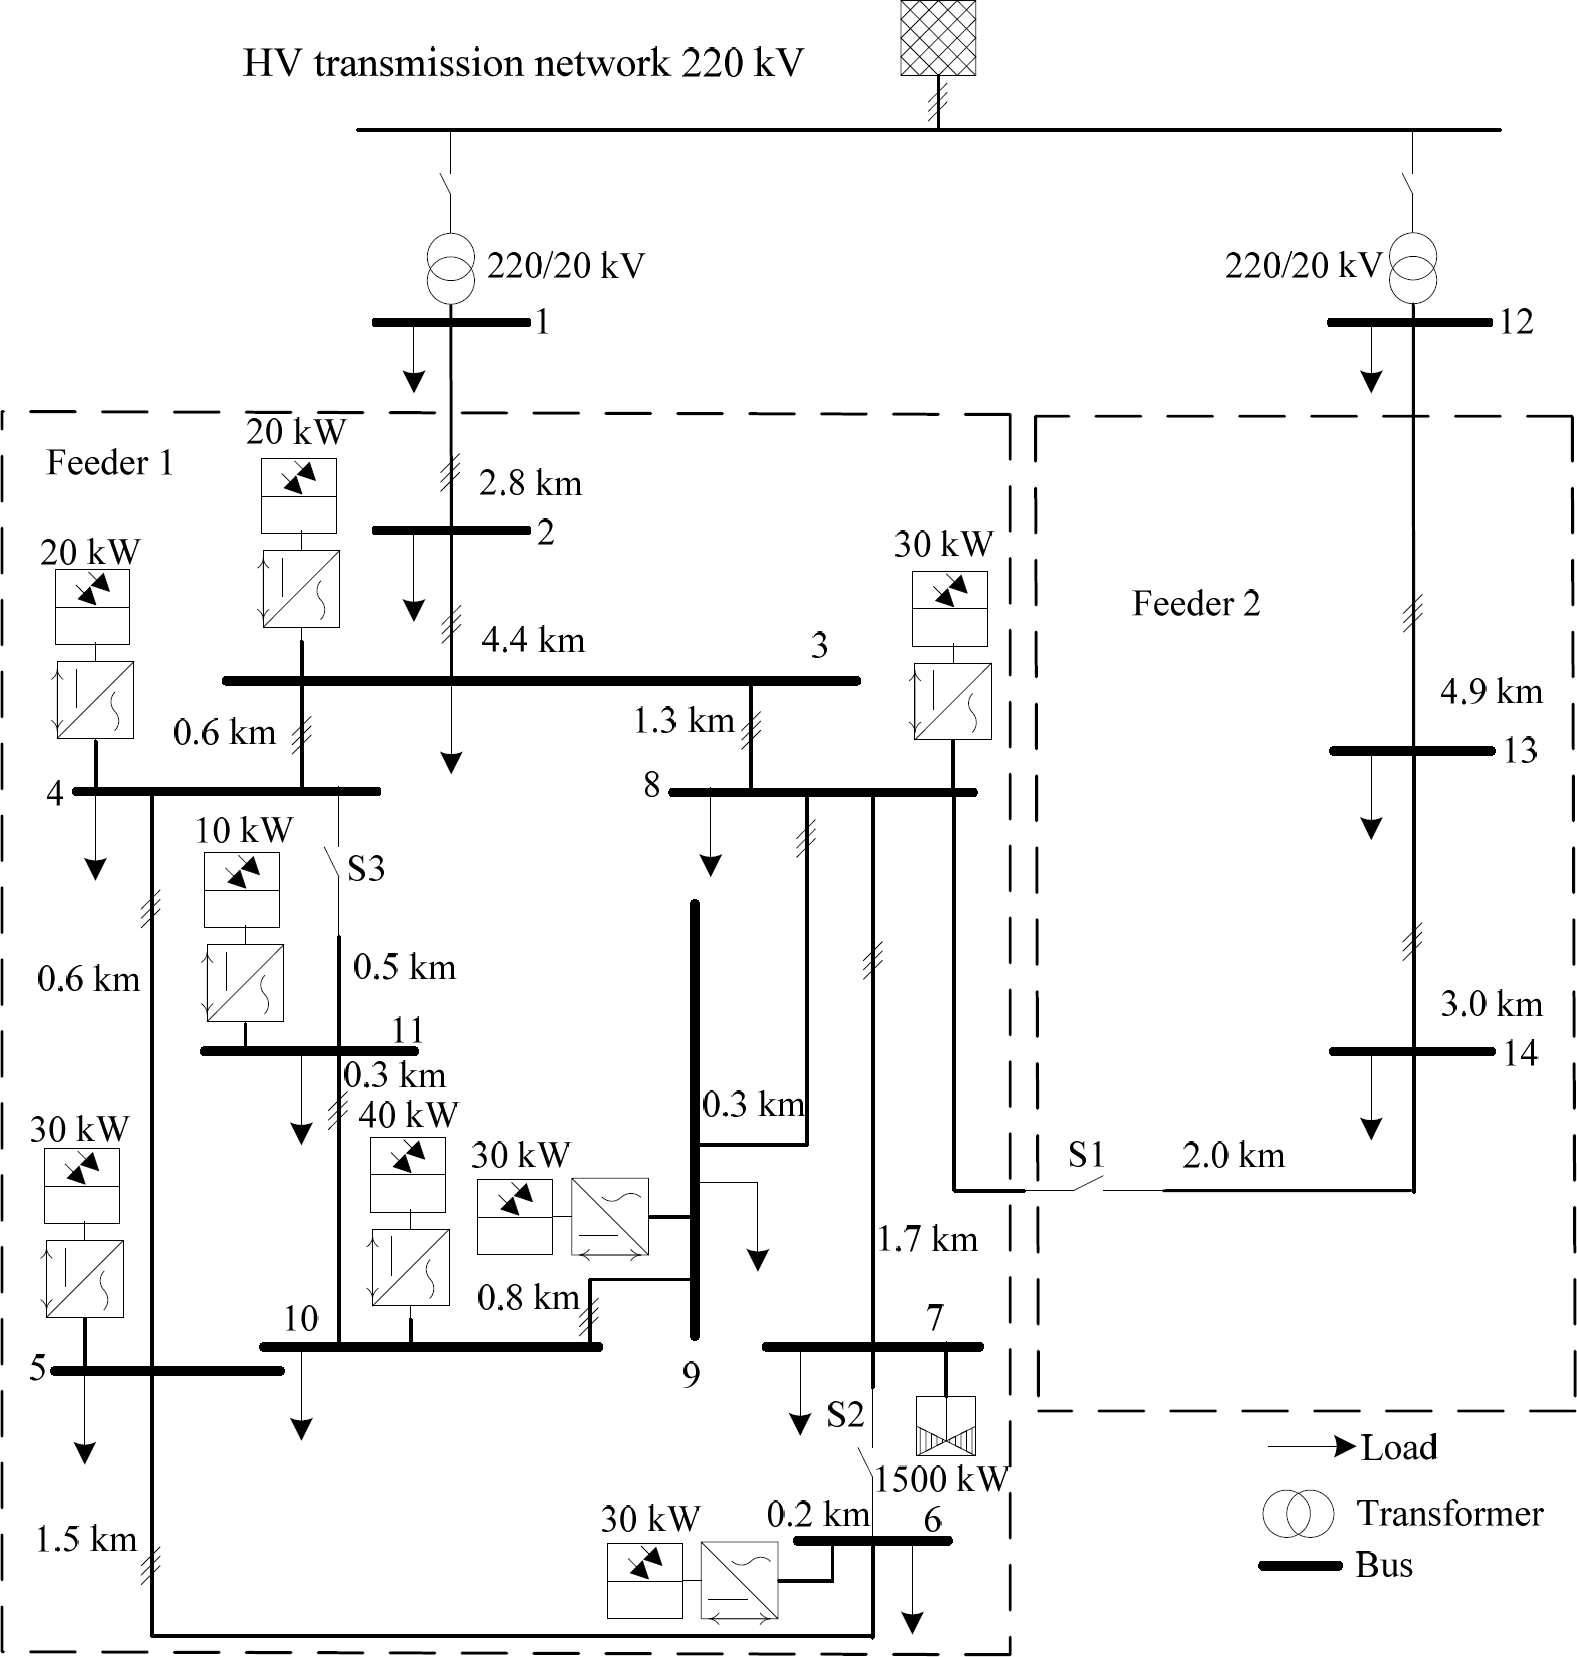
\includegraphics[height=14cm, width=13.5cm]{figures/cigre_network_mv_der.png}
    \caption[size = 9]{CIGRE network with solar and wind power that is used in the reinforcement learning algorithm}
    \label{fig:problem:cigre_network}
\end{figure}
The left-most feeder has several solar producing units connected and wind power connected to bus 7. 



\end{document}